\subsection{Esercizio 30}
Tabulare il numero di valutazioni di funzione richieste dalle function
degli Esercizi 29 e 30 per approssimare l'integral
\[
    I(f) = \int_{0}^{1} sin\left(\frac{1}{0.01+x}\right)\,dx,
\]
con tolleranze $tol$ = $10^{-2}$, $10^{-3}$, $10^{-4}$, $10^{-5}$, $10^{-6}$.
\newline \textbf{Soluzione:}

Eseguendo lo script \nameref{cod:30} si ottengono i risultati contenuti nella
tabella \ref{tab:30} e nella figura \ref{fig:es30}.
\begin{table}[ht]
    \centering
    \renewcommand\arraystretch{2}
    \begin{tabular}{| l | c c c c c |}
        \hline
        Metodo           & $10^{-2}$ & $10^{-3}$ & $10^{-4}$ & $10^{-5}$ & $10^{-6}$ \\
        \hline
        adattivo trapezi & 303       & 991       & 3119      & 10123     & 31837     \\
        adattivo Simpson & 85        & 185       & 341       & 625       & 1081      \\
        \hline
    \end{tabular}
    \caption{Numero di valutazioni funzionali rispetto a grado e tolleranza per approssimare l'integrale}
    \label{tab:30}
\end{table}
\FloatBarrier
\begin{figure}[!ht]
    \centering
    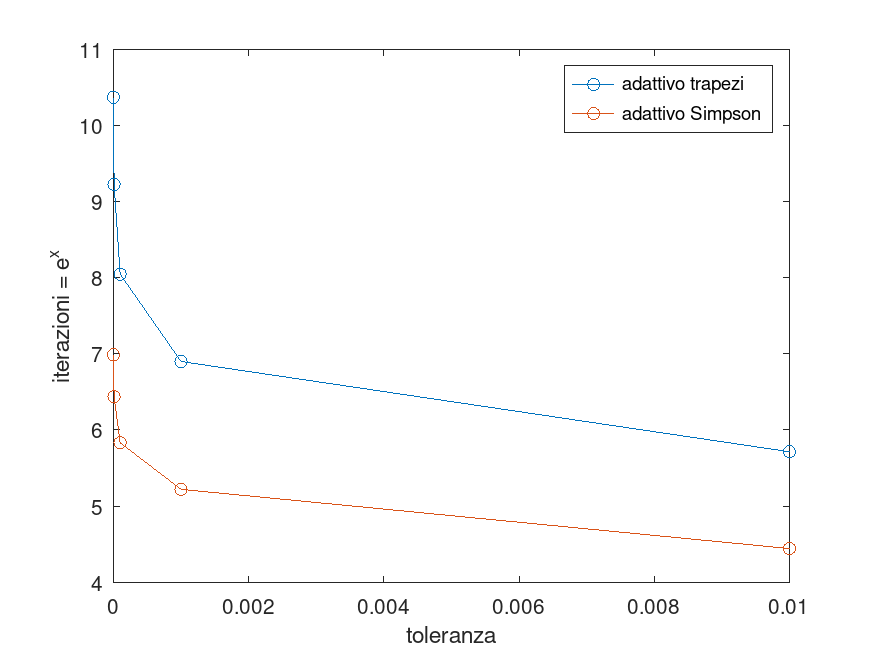
\includegraphics[width=16cm,height=10cm,keepaspectratio]{capitolo5/es30_figure.png}
    \caption{Numero di valutazioni funzionali rispetto tolleranza per approssimare l'integrale}
    \label{fig:es30}
\end{figure}
\FloatBarrier
